\documentclass[journal,11pt,onecolumn]{IEEEtran}

% Page configurations
\title{ME: MECHANICAL ENGINEERING}
\usepackage[a4paper,bottom=1in,top=1in]{geometry}
\usepackage{amsmath}
\usepackage{graphicx}
\usepackage{float}
\usepackage{tikz}
\usepackage{multicol}
\usepackage{tfrupee}
\setlength{\columnsep}{1cm}
\usepackage{gvv}
\usetikzlibrary{arrows}
\usetikzlibrary{decorations.markings}
\graphicspath{{figs/}}

\begin{document}

\begin{center}
    \Large
    \textbf{ME: MECHANICAL ENGINEERING}
\end{center}

\textit{Duration} : Three hours
\hfill
\textit{Maximum Marks} : 100

% \\\\

\textbf{Read the following instructions carefully}

\begin{enumerate}
    \item Do not open the seal of the Question Booklet until you are asked to do so by the invigilator.

    \item Take out the Optical Response Sheet (ORS) from this Question Booklet without breaking the seal and read the instructions printed on the ORS carefully. If you find that the Question Booklet Code printed at the right hand top corner of this page does not match with the Booklet Code on the ORS, exchange the booklet immediately with a new sealed Question Booklet.

    \item On the right half of the ORS, using ONLY a black ink ball point pen, (i) darken the bubble corresponding to your test paper code and the appropriate bubble under each digit of your registration number and (ii) write your registration number, your name and name of the examination centre and put your signature at the specified location.

    \item This Question Booklet contains 16 pages including blank pages for rough work. After you are permitted to open the seal, please check all pages and report discrepancies, if any, to the invigilator.

    \item There are a total of 65 questions carrying 100 marks. All these questions are of objective type. Each question has only one correct answer. Questions must be answered on the left hand side of the ORS by darkening the appropriate bubble (marked A, B, C, D) using ONLY a black ink ball point pen against the question number. For each question darken the bubble of the correct answer. More than one answer bubbled against a question will be treated as an incorrect response.

    \item Since bubbles darkened by the black ink ball point pen cannot be erased, candidates should darken the bubbles in the ORS very carefully.

    \item Questions Q.1 -- Q.25 carry 1 mark each. Questions Q.26 -- Q.55 carry 2 marks each. The 2 marks questions include two pairs of common data questions and two pairs of linked answer questions. The answer to the second question of the linked answer questions depends on the answer to the first question of the pair. If the first question in the linked pair is wrongly answered or is unattempted, then the answer to the second question in the pair will not be evaluated.

    \item Questions Q.56 -- Q.65 belong to General Aptitude (GA) section and carry a total of 15 marks. Questions Q.56 -- Q.60 carry 1 mark each, and questions Q.61 -- Q.65 carry 2 marks each.

    \item Unattempted questions will result in zero mark and wrong answers will result in NEGATIVE marks. For all 1 mark questions, 1/3 mark will be deducted for each wrong answer. For all 2 marks questions, 2/3 mark will be deducted for each wrong answer. However, in the case of the linked answer question pair, there will be negative marks only for wrong answer to the first question and no negative marks for wrong answer to the second question.

    \item Calculator is allowed whereas charts, graph sheets or tables are NOT allowed in the examination hall.

    \item Rough work can be done on the question paper itself. Blank pages are provided at the end of the question paper for rough work.

    \item Before the start of the examination, write your name and registration number in the space provided below using a black ink ball point pen.
\end{enumerate}

\textbf{Name:} \underline{\hspace{6cm}}

\textbf{Registration Number:} \underline{\hspace{4cm}}

\newpage

\large\textbf{Q.1 -- Q.25 carry one mark each.}\\

\begin{enumerate}

    \item In abrasive jet machining, as the distance between the nozzle tip and the work surface increases, the material removal rate

          \begin{enumerate}
              \item increases continuously.
              \item decreases continuously
              \item decreases, becomes stable and then increases.
              \item increases, becomes stable and then decreases.
          \end{enumerate}

    \item Match the following metal forming processes with their associated stresses in the workpiece.

          \begin{table}[H]
              \centering
              \begin{tabular}{|l|l|l|l|}
                  \hline
                  \textbf{Metal forming process} &  & \textbf{Type of stress}    & \\
                  \hline
                  1. Coining                     &  & P. Tensile                 & \\
                  2. Wire Drawing                &  & Q. Shear                   & \\
                  3. Blanking                    &  & R. Tensile and compressive & \\
                  4. Deep Drawing                &  & S. Compressive             & \\
                  \hline
              \end{tabular}
          \end{table}

          \begin{enumerate}
              \begin{multicols}{2}
                  \item 1-S, 2-P, 3-Q, 4-R
                  \item 1-S, 2-P, 3-R, 4-Q
                  \item 1-P, 2-Q, 3-S, 4-R
                  \item 1-P, 2-R, 3-Q, 4-S
              \end{multicols}
          \end{enumerate}

    \item In an interchangeable assembly, shafts of size $25.000^{+0.040}_{-0.010}$ mm mate with holes of size \(25.000^{+0.030}_{+0.020}\) mm. The maximum interference (in \textit{microns}) in the assembly is

          \begin{enumerate}
              \begin{multicols}{4}
                  \item 40
                  \item 30
                  \item 20
                  \item 10
              \end{multicols}
          \end{enumerate}

    \item During normalizing process of steel, the specimen is heated

          \begin{enumerate}
              \item between the upper and lower critical temperature and cooled in still air.
              \item above the upper critical temperature and cooled in furnace.
              \item above the upper critical temperature and cooled in still air.
              \item between the upper and lower critical temperature and cooled in furnace.
          \end{enumerate}

    \item Oil flows through a 200 mm diameter horizontal cast iron pipe (friction factor, f = 0.0225) of length 500 m. The volumetric flow rate is 0.2 m³/s. The head loss (in m) due to friction is (assume g = 9.81 m/s²)

          \begin{enumerate}
              \begin{multicols}{4}
                  \item 116.18
                  \item 0.116
                  \item 18.22
                  \item 232.36
              \end{multicols}
          \end{enumerate}

    \item For an opaque surface, the absorptivity \(\alpha\), transmissivity \(\tau\) and reflectivity \(\rho\) are related by the equation:

          \begin{enumerate}
              \begin{multicols}{4}
                  \item \(\alpha + \tau + \rho = 1\)
                  \item \(\alpha = \tau + \rho = 0\)\columnbreak
                  \item \(\alpha + \rho = 1\)
                  \item \(\alpha = \tau = \rho = 0\)
              \end{multicols}
          \end{enumerate}

    \item Steam enters an adiabatic turbine operating at steady state with an enthalpy of 3251.0 kJ/kg and leaves as a saturated mixture at 15 kPa with quality (dryness fraction) 0.9. The enthalpies of the saturated liquid and vapor at 15 kPa are \(h_f = 225.94\) kJ/kg and \(h_g = 2598.3\) kJ/kg respectively. The mass flow rate of steam is 10 kg/s. Kinetic and potential energy changes are negligible. The power output of the turbine in MW is

          \begin{enumerate}
              \begin{multicols}{4}
                  \item 6.5
                  \item 8.9
                  \item 9.1
                  \item 27.0
              \end{multicols}
          \end{enumerate}

    \item The following are the data for two crossed helical gears used for speed reduction:\\
          Gear I: Pitch circle diameter in the plane of rotation 80 mm and helix angle 30°\\
          Gear II: Pitch circle diameter in the plane of rotation 120 mm and helix angle 22.5°\\
          If the input speed is 1440 rpm, the output speed in rpm is

          \begin{enumerate}
              \begin{multicols}{4}
                  \item 1200
                  \item 900
                  \item 875
                  \item 720
              \end{multicols}
          \end{enumerate}

    \item A solid disc of radius r rolls without slipping on a horizontal floor with angular velocity \(\omega\) and angular acceleration \(\alpha\). The magnitude of the acceleration of the point of contact on the disc is

          \begin{enumerate}
              \begin{multicols}{4}
                  \item zero
                  \item \(r\alpha\)
                  \item \(\sqrt{(r\alpha)^2 + (r\omega^2)^2}\)
                  \item \(r\omega^2\)
              \end{multicols}
          \end{enumerate}

    \item A thin walled spherical shell is subjected to an internal pressure. If the radius of the shell is increased by 1\% and the thickness is reduced by 1\%, with the internal pressure remaining the same, the percentage change in the circumferential (hoop) stress is

          \begin{enumerate}
              \begin{multicols}{4}
                  \item 0
                  \item 1
                  \item 1.08
                  \item 2.02
              \end{multicols}
          \end{enumerate}

    \item The area enclosed between the straight line y = x and the parabola \(y = x^2\) in the x-y plane is

          \begin{enumerate}
              \begin{multicols}{4}
                  \item 1/6
                  \item 1/4
                  \item 1/3
                  \item 1/2
              \end{multicols}
          \end{enumerate}

    \item Consider the function \(f(x) = |x|\) in the interval \(-1 \leq x \leq 1\). At the point x = 0, f(x) is

          \begin{enumerate}
              \item continuous and differentiable.
              \item non-continuous and differentiable.
              \item continuous and non-differentiable.
              \item neither continuous nor differentiable.
          \end{enumerate}

    \item Which one of the following is NOT a decision taken during the aggregate production planning stage?

          \begin{enumerate}
              \begin{multicols}{2}
                  \item Scheduling of machines
                  \item Amount of labour to be committed\columnbreak
                  \item Rate at which production should happen
                  \item Inventory to be carried forward
              \end{multicols}
          \end{enumerate}

    \item \(\lim_{x \to 0} \frac{1-\cos x}{x^2}\) is

          \begin{enumerate}
              \begin{multicols}{4}
                  \item 1/4
                  \item 1/2
                  \item 1
                  \item 2
              \end{multicols}
          \end{enumerate}

    \item A CNC vertical milling machine has to cut a straight slot of 10 mm width and 2 mm depth by a cutter of 10 mm diameter between points (0, 0) and (100, 100) on the XY plane (dimensions in mm). The feed rate used for milling is 50 mm/min. Milling time for the slot (in seconds) is

          \begin{enumerate}
              \begin{multicols}{4}
                  \item 120
                  \item 170
                  \item 180
                  \item 240
              \end{multicols}
          \end{enumerate}

    \item A solid cylinder of diameter 100 mm and height 50 mm is forged between two frictionless flat dies to a height of 25 mm. The percentage change in diameter is

          \begin{enumerate}
              \begin{multicols}{4}
                  \item 0
                  \item 2.07
                  \item 20.7
                  \item 41.4
              \end{multicols}
          \end{enumerate}

    \item The velocity triangles at the inlet and exit of the rotor of a turbomachine are shown. V denotes the absolute velocity of the fluid, W denotes the relative velocity of the fluid and U denotes the blade velocity. Subscripts 1 and 2 refer to inlet and outlet respectively. If \(V_2 = W_1\) and \(V_1 = W_2\), then the degree of reaction is

          \begin{figure}[H]
              \centering
              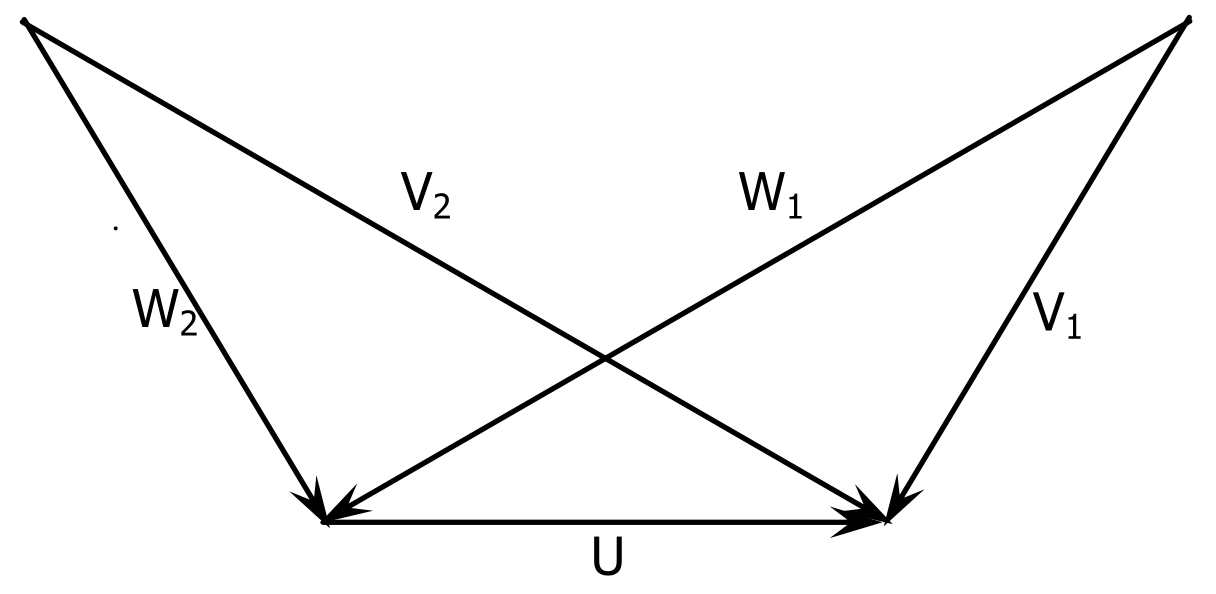
\includegraphics[scale=0.2]{q17}
              \caption{}
              \label{q17}
          \end{figure}

          \begin{enumerate}
              \begin{multicols}{4}
                  \item 0
                  \item 1
                  \item 0.5
                  \item 0.25
              \end{multicols}
          \end{enumerate}

    \item Which one of the following configurations has the highest fin effectiveness?

          \begin{enumerate}
              \begin{multicols}{2}
                  \item Thin, closely spaced fins
                  \item Thin, widely spaced fins
                  \item Thick, widely spaced fins
                  \item Thick, closely spaced fins
              \end{multicols}
          \end{enumerate}

    \item An ideal gas of mass m and temperature \(T_1\) undergoes a reversible isothermal process from an initial pressure \(P_1\) to final pressure \(P_2\). The heat loss during the process is Q. The entropy change \(\Delta S\) of the gas is

          \begin{enumerate}
              \begin{multicols}{2}
                  \item \(mR \ln\left(\frac{P_2}{P_1}\right)\)
                  \item \(mR \ln\left(\frac{P_1}{P_2}\right)\)
                  \item \( mR \ln\left(\frac{P_2}{P_1}\right) - \frac{Q}{T_1}\)
                  \item zero
              \end{multicols}
          \end{enumerate}

    \item In the mechanism given below, if the angular velocity of the eccentric circular disc is 1 rad/s, the angular velocity (rad/s) of the follower link for the instant shown in the figure is
          \textit{Note: All dimensions are in mm.}
          \begin{figure}[H]
              \centering
              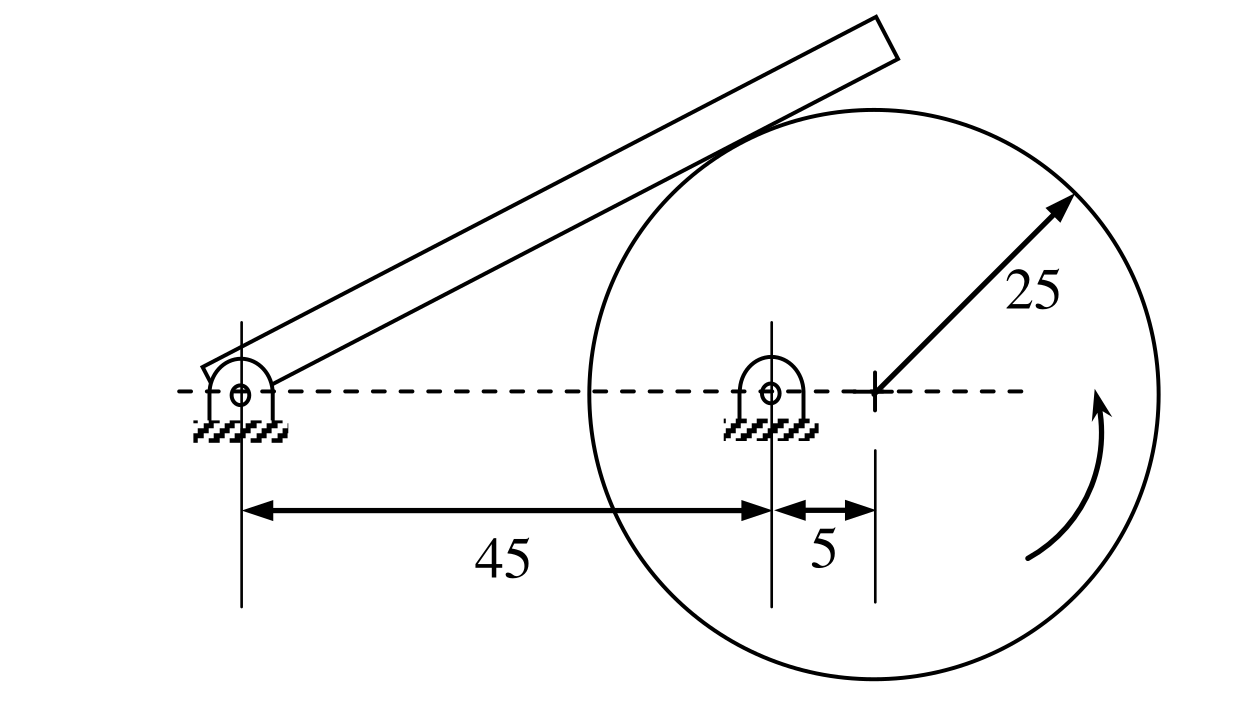
\includegraphics[scale=0.2]{q20}
              \caption{}
              \label{q20}
          \end{figure}


          \begin{enumerate}
              \begin{multicols}{4}
                  \item 0.05
                  \item 0.1
                  \item 5.0
                  \item 10.0
              \end{multicols}
          \end{enumerate}

    \item A circular solid disc of uniform thickness 20 mm, radius 200 mm and mass 20 kg, is used as a flywheel. If it rotates at 600 rpm, the kinetic energy of the flywheel, in Joules is

          \begin{enumerate}
              \begin{multicols}{4}
                  \item 395
                  \item 790
                  \item 1580
                  \item 3160
              \end{multicols}
          \end{enumerate}

    \item A cantilever beam of length L is subjected to a moment M at the free end. The moment of inertia of the beam cross section about the neutral axis is I and the Young's modulus is E. The magnitude of the maximum deflection is

          \begin{enumerate}
              \begin{multicols}{4}
                  \item \(\frac{ML^2}{2EI}\)
                  \item \(\frac{ML^2}{EI}\)
                  \item \(\frac{2ML^2}{EI}\)
                  \item \(\frac{4ML^2}{EI}\)
              \end{multicols}
          \end{enumerate}

    \item For a long slender column of uniform cross section, the ratio of critical buckling load for the case with both ends clamped to the case with both ends hinged is

          \begin{enumerate}
              \begin{multicols}{4}
                  \item 1
                  \item 2
                  \item 4
                  \item 8
              \end{multicols}
          \end{enumerate}

    \item At x = 0, the function \(f(x) = \frac{x^3}{1+x^2}\) has

          \begin{enumerate}
              \begin{multicols}{4}
                  \item a maximum value
                  \item a minimum value
                  \item a singularity
                  \item a point of inflection
              \end{multicols}
          \end{enumerate}

    \item For the spherical surface \(x^2 + y^2 + z^2 = 1\), the unit outward normal vector at the point \(\left(\frac{1}{2}, \frac{1}{2}, 0\right)\) is given by

          \begin{enumerate}
              \begin{multicols}{4}
                  \item \(\frac{1}{2}\hat{i} + \frac{1}{2}\hat{j}\)
                  \item \(-\frac{1}{2}\hat{i} - \frac{1}{2}\hat{j}\)
                  \item \(\hat{k}\)
                  \item \(\frac{1}{\sqrt{3}}\hat{i} + \frac{1}{\sqrt{3}}\hat{j} + \frac{1}{\sqrt{3}}\hat{k}\)
              \end{multicols}
          \end{enumerate}

\end{enumerate}

\newpage

\large\textbf{Q.26 -- Q.55 carry two marks each.}\\

\begin{enumerate}[resume]

    \item The homogeneous state of stress for a metal part undergoing plastic deformation is
          \[T = \myvec{10 & 5 & 0 \\ 5 & 20 & 0 \\ 0 & 0 & 10}\]
          where the stress component values are in MPa. Using von Mises yield criterion, the value of estimated shear yield stress, in MPa is

          \begin{enumerate}
              \begin{multicols}{4}
                  \item 9.50
                  \item 16.07
                  \item 28.52
                  \item 49.41
              \end{multicols}
          \end{enumerate}

    \item Details pertaining to an orthogonal metal cutting process are given below.

          \begin{table}[H]
              \centering
              \begin{tabular}{|l|l|}
                  \hline
                  Chip thickness ratio                 & 0.4        \\
                  \hline
                  Undeformed thickness                 & 0.6 mm     \\
                  \hline
                  Rake angle                           & +10°       \\
                  \hline
                  Cutting speed                        & 2.5 m/s    \\
                  \hline
                  Mean thickness of primary shear zone & 25 microns \\
                  \hline
              \end{tabular}
          \end{table}

          The shear strain rate in s$^{-1}$ during the process is

          \begin{enumerate}
              \begin{multicols}{4}
                  \item \(0.1781 \times 10^5\)
                  \item \(0.7754 \times 10^5\)
                  \item \(1.0104 \times 10^5\)
                  \item \(4.397 \times 10^5\)
              \end{multicols}
          \end{enumerate}

    \item In a single pass drilling operation, a through hole of 15 mm diameter is to be drilled in a steel plate of 50 mm thickness. Drill spindle speed is 500 rpm, feed is 0.2 mm/rev and drill point angle is 118°. Assuming 2 mm clearance at approach and exit, the total drill time (in seconds) is

          \begin{enumerate}
              \begin{multicols}{4}
                  \item 35.1
                  \item 32.4
                  \item 31.2
                  \item 30.1
              \end{multicols}
          \end{enumerate}

    \item Consider two infinitely long thin concentric tubes of circular cross section as shown in the figure. If \(D_1\) and \(D_2\) are the diameters of the inner and outer tubes respectively, then the view factor \(F_{22}\) is given by
          \begin{figure}[H]
              \centering
              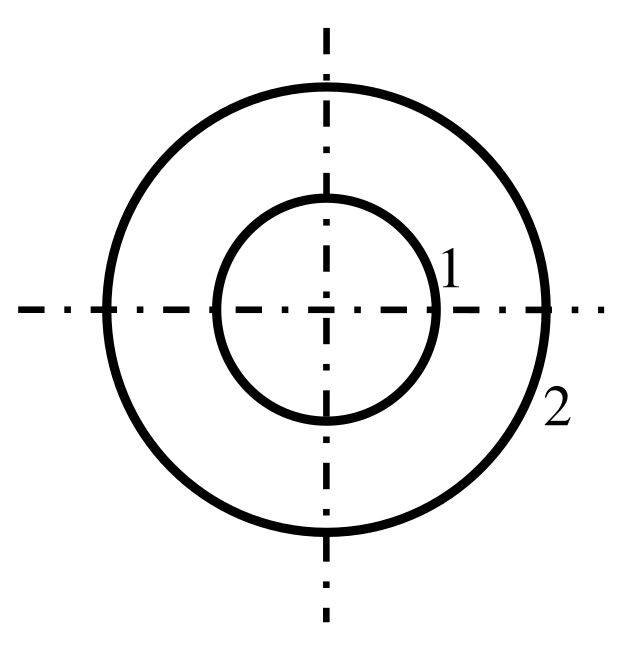
\includegraphics[scale=0.2]{q29}
              \caption{}
              \label{q29}
          \end{figure}

          \begin{enumerate}
              \begin{multicols}{4}
                  \item \(1 - \frac{D_1}{D_2}\)
                  \item zero
                  \item \(\frac{D_1}{D_2}\)
                  \item \(1 - \frac{D_1}{D_2}\)
              \end{multicols}
          \end{enumerate}

    \item An incompressible fluid flows over a flat plate with zero pressure gradient. The boundary layer thickness is 1 mm at a location where the Reynolds number is 1000. If the velocity of the fluid alone is increased by a factor of 4, then the boundary layer thickness at the same location, in mm will be

          \begin{enumerate}
              \begin{multicols}{4}
                  \item 4
                  \item 2
                  \item 0.5
                  \item 0.25
              \end{multicols}
          \end{enumerate}

    \item A room contains 35 kg of dry air and 0.5 kg of water vapor. The total pressure and temperature of air in the room are 100 kPa and 25°C respectively. Given that the saturation pressure for water at 25°C is 3.17 kPa, the relative humidity of the air in the room is

          \begin{enumerate}
              \begin{multicols}{4}
                  \item 67\%
                  \item 55\%
                  \item 83\%
                  \item 71\%
              \end{multicols}
          \end{enumerate}

    \item A fillet welded joint is subjected to transverse loading F as shown in the figure. Both legs of the fillets are of 10 mm size and the weld length is 30 mm. If the allowable shear stress of the weld is 94 MPa, considering the minimum throat area of the weld, the maximum allowable transverse load in kN is
          \begin{figure}[H]
              \centering
              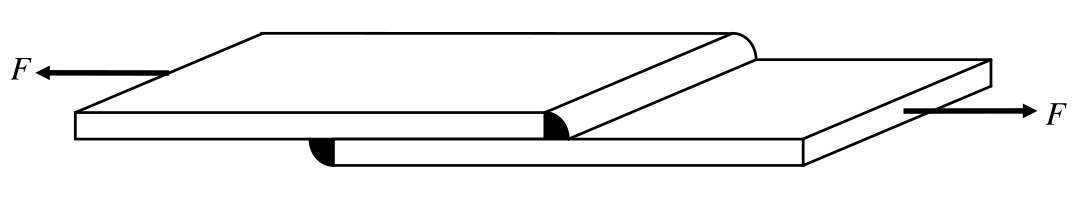
\includegraphics[scale=0.2]{q32}
              \caption{}
              \label{q32}
          \end{figure}
          \begin{enumerate}
              \begin{multicols}{4}
                  \item 14.44
                  \item 17.92
                  \item 19.93
                  \item 22.16
              \end{multicols}
          \end{enumerate}

    \item A concentrated mass m is attached at the centre of a rod of length 2L as shown in the figure. The rod is kept in a horizontal equilibrium position by a spring of stiffness k. For very small amplitude of vibration, neglecting the weights of the rod and spring, the undamped natural frequency of the system is
          \begin{figure}[H]
              \centering
              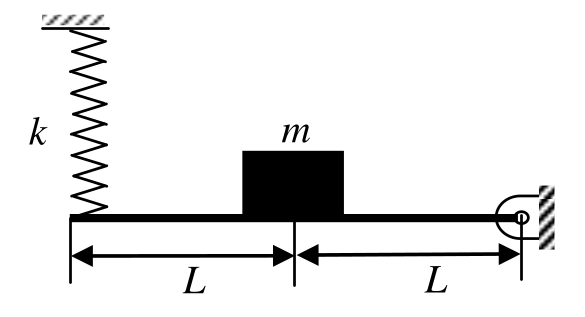
\includegraphics[scale=0.2]{q33}
              \caption{}
              \label{q33}
          \end{figure}

          \begin{enumerate}
              \begin{multicols}{4}
                  \item \(\sqrt{\frac{k}{m}}\)
                  \item \(\sqrt{\frac{2k}{m}}\)
                  \item \(\sqrt{\frac{k}{2m}}\)
                  \item \(\sqrt{\frac{4k}{m}}\)
              \end{multicols}
          \end{enumerate}

    \item The state of stress at a point under plane stress condition is
          \[\sigma_{xx} = 40 \text{ MPa}, \quad \sigma_{yy} = 100 \text{ MPa} \quad \text{and} \quad \tau_{xy} = 40 \text{ MPa}\]
          The radius of the Mohr's circle representing the given state of stress in MPa is

          \begin{enumerate}
              \begin{multicols}{4}
                  \item 40
                  \item 50
                  \item 60
                  \item 100
              \end{multicols}
          \end{enumerate}

    \item The inverse Laplace transform of the function \(F(s) = \frac{1}{s(s+1)}\) is given by

          \begin{enumerate}
              \begin{multicols}{4}
                  \item \(f(t) = \sin t\)
                  \item \(f(t) = e^{-t} \sin t\)
                  \item \(f(t) = e^{-t}\)
                  \item \(f(t) = 1 - e^{-t}\)
              \end{multicols}
          \end{enumerate}

    \item For the matrix \(A = \myvec{5 & 3 \\ 1 & 3}\), ONE of the normalized eigen vectors is given as

          \begin{enumerate}
              \begin{multicols}{4}
                  \item \(\myvec{\frac{3}{2} \\ \frac{1}{2}}\)
                  \item \(\myvec{\frac{1}{\sqrt{2}} \\ -\frac{1}{\sqrt{2}}}\)
                  \item \(\myvec{\frac{3}{\sqrt{10}} \\ \frac{1}{\sqrt{10}}}\)
                  \item \(\myvec{\frac{1}{\sqrt{5}} \\ \frac{2}{\sqrt{5}}}\)
              \end{multicols}
          \end{enumerate}

    \item Calculate the punch size in mm, for a circular blanking operation for which details are given below.

          \begin{table}[H]
              \centering
              \begin{tabular}{|l|l|}
                  \hline
                  Size of the blank                      & 25 mm   \\
                  \hline
                  Thickness of the sheet                 & 2 mm    \\
                  \hline
                  Radial clearance between punch and die & 0.06 mm \\
                  \hline
                  Die allowance                          & 0.05 mm \\
                  \hline
              \end{tabular}
          \end{table}

          \begin{enumerate}
              \begin{multicols}{4}
                  \item 24.83
                  \item 24.89
                  \item 25.01
                  \item 25.17
              \end{multicols}
          \end{enumerate}

    \item In a single pass rolling process using 410 mm diameter steel rollers, a strip of width 140 mm and thickness 8 mm undergoes 10\% reduction of thickness. The angle of bite in radians is

          \begin{enumerate}
              \begin{multicols}{4}
                  \item 0.006
                  \item 0.031
                  \item 0.062
                  \item 0.600
              \end{multicols}
          \end{enumerate}

    \item In a DC arc welding operation, the voltage-arc length characteristic was obtained as \(V_{arc} = 20 + 5l\) where the arc length l was varied between 5 mm and 7 mm. Here \(V_{arc}\) denotes the arc voltage in Volts. The arc current was varied from 400 A to 500 A. Assuming linear power source characteristic, the open circuit voltage and the short circuit current for the welding operation are
          \begin{enumerate}
              \begin{multicols}{2}
                  \item 45 V, 450 A
                  \item 75 V, 750 A
                  \item 95 V, 950 A
                  \item 150 V, 1500 A
              \end{multicols}
          \end{enumerate}

    \item A large tank with a nozzle attached contains three immiscible, inviscid fluids as shown. Assuming that the changes in \(h_1\), \(h_2\) and \(h_3\) are negligible, the instantaneous discharge velocity is
          \begin{figure}[H]
              \centering
              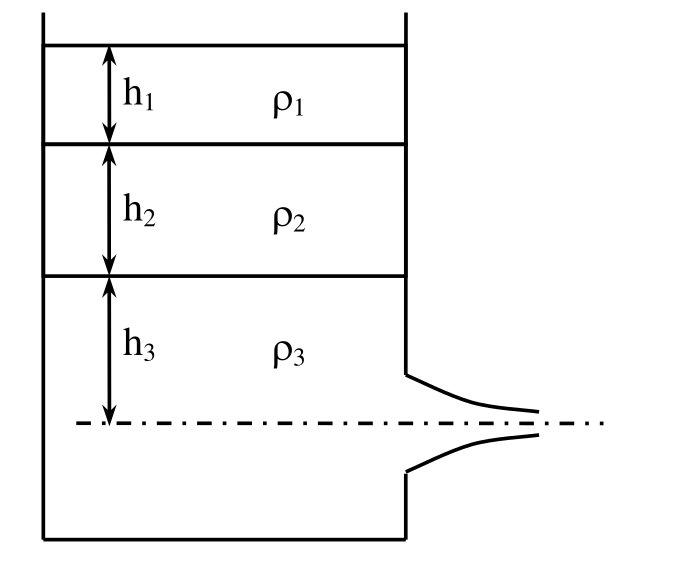
\includegraphics[scale=0.2]{q40}
              \caption{}
              \label{q40}
          \end{figure}

          \begin{enumerate}
              \begin{multicols}{2}
                  \item \(\sqrt{2gh_3\left(\frac{\rho_1 h_1 + \rho_2 h_2 + \rho_3 h_3}{\rho_3 h_3}\right)}\)
                  \item \(\sqrt{2g(h_1 + h_2 + h_3)}\)
                  \item \(\sqrt{2g\left(\frac{\rho_1 h_1 + \rho_2 h_2 + \rho_3 h_3}{\rho_1 + \rho_2 + \rho_3}\right)}\)
                  \item \(\sqrt{2g\left(\frac{(\rho_1-\rho_3)h_1 + (\rho_2-\rho_3)h_2}{\rho_3} + h_1 + h_2 + h_3\right)}\)
              \end{multicols}
          \end{enumerate}

    \item Water (\(C_p = 4.18\) kJ/kg.K) at 80°C enters a counterflow heat exchanger with a mass flow rate of 0.5 kg/s. Air (\(C_p = 1\) kJ/kg.K) enters at 30°C with a mass flow rate of 2.09 kg/s. If the effectiveness of the heat exchanger is 0.8, the LMTD (in °C) is

          \begin{enumerate}
              \begin{multicols}{4}
                  \item 40
                  \item 20
                  \item 10
                  \item 5
              \end{multicols}
          \end{enumerate}

    \item A solid steel cube constrained on all six faces is heated so that the temperature rises uniformly by \(\Delta T\). If the thermal coefficient of the material is \(\alpha\), Young's modulus is E and the Poisson's ratio is \(\nu\), the thermal stress developed in the cube due to heating is

          \begin{enumerate}
              \begin{multicols}{4}
                  \item \(\frac{\alpha(\Delta T) E}{(1-2\nu)}\)
                  \item \(\frac{2\alpha(\Delta T) E}{(1-2\nu)}\)
                  \item \(\frac{3\alpha(\Delta T) E}{(1-2\nu)}\)
                  \item \(\frac{\alpha(\Delta T) E}{3(1-2\nu)}\)
              \end{multicols}
          \end{enumerate}

    \item A solid circular shaft needs to be designed to transmit a torque of 50 N.m. If the allowable shear stress of the material is 140 MPa, assuming a factor of safety of 2, the minimum allowable design diameter in mm is
          \begin{enumerate}
              \begin{multicols}{4}
                  \item 8
                  \item 16
                  \item 24
                  \item 32
              \end{multicols}
          \end{enumerate}

    \item A force of 400 N is applied to the brake drum of 0.5 m diameter in a band-brake system as shown in the figure, where the wrapping angle is 180°. If the coefficient of friction between the drum and the band is 0.25, the braking torque applied, in N.m is
          \begin{figure}[H]
              \centering
              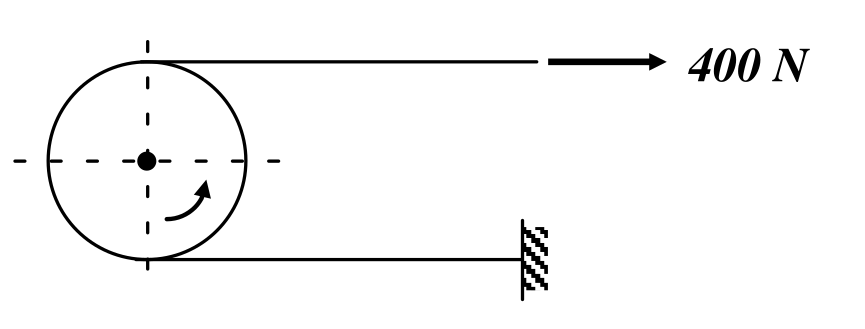
\includegraphics[scale=0.2]{q44}
              \caption{}
              \label{q44}
          \end{figure}

          \begin{enumerate}
              \begin{multicols}{4}
                  \item 100.6
                  \item 54.4
                  \item 22.1
                  \item 15.7
              \end{multicols}
          \end{enumerate}

    \item A box contains 4 red balls and 6 black balls. Three balls are selected randomly from the box one after another, without replacement. The probability that the selected set contains one red ball and two black balls is

          \begin{enumerate}
              \begin{multicols}{4}
                  \item 1/20
                  \item 1/12
                  \item 3/10
                  \item 1/2
              \end{multicols}
          \end{enumerate}

    \item Consider the differential equation \(x^2\frac{d^2y}{dx^2} + x\frac{dy}{dx} - 4y = 0\) with the boundary conditions of \(y(0) = 0\) and \(y(1) = 1\). The complete solution of the differential equation is

          \begin{enumerate}
              \begin{multicols}{4}
                  \item \(x^2\)
                  \item \(\sin\left(\frac{\pi x}{2}\right)\)
                  \item \(e^x \sin\left(\frac{\pi x}{2}\right)\)
                  \item \(e^{-x} \sin\left(\frac{\pi x}{2}\right)\)
              \end{multicols}
          \end{enumerate}

    \item
          \begin{align}
              2x + 4y + z & = 2 \\
              x + 2y + 5z & = 1 \\
              x + 2y + z  & = 1
          \end{align}

          The system of algebraic equations given above has


          \begin{enumerate}
              \item a unique solution of x = 1, y = 1 and z = 1.
              \item only the two solutions of (x = 1, y = 1, z = 1) and (x = 2, y = 1, z = 0).
              \item infinite number of solutions.
              \item no feasible solution.
          \end{enumerate}

\end{enumerate}

\newpage

\large\textbf{Common Data Questions}\\

\normalsize\textbf{Common Data for Questions 48 and 49:}

Two steel truss members, AC and BC, each having cross sectional area of 100 mm², are subjected to a horizontal force F as shown in figure. All the joints are hinged.

\begin{figure}[H]
    \centering
    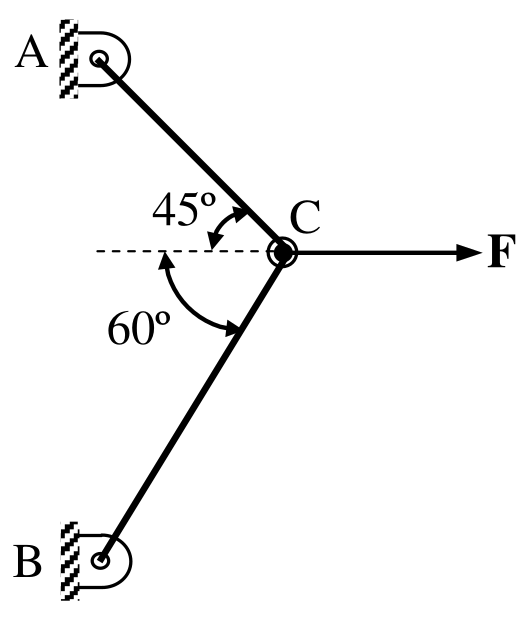
\includegraphics[scale=0.2]{q48}
    \caption{}
    \label{q48}
\end{figure}
\begin{enumerate}[resume]

    \item If F = 1 kN, the magnitude of the vertical reaction force developed at the point B in kN is

          \begin{enumerate}
              \begin{multicols}{4}
                  \item 0.63
                  \item 0.32
                  \item 1.26
                  \item 1.46
              \end{multicols}
          \end{enumerate}

    \item The maximum force F in kN that can be applied at C such that the axial stress in any of the truss members DOES NOT exceed 100 MPa is

          \begin{enumerate}
              \begin{multicols}{4}
                  \item 8.17
                  \item 11.15
                  \item 14.14
                  \item 22.30
              \end{multicols}
          \end{enumerate}

\end{enumerate}

\normalsize\textbf{Common Data for Questions 50 and 51:}

A refrigerator operates between 120 kPa and 800 kPa in an ideal vapor compression cycle with R-134a as the refrigerant. The refrigerant enters the compressor as saturated vapor and leaves the condenser as saturated liquid. The mass flow rate of the refrigerant is 0.2 kg/s. Properties for R-134a are as follows:

\begin{table}[H]
    \centering
    \begin{tabular}{|l|l|l|l|l|l|}
        \hline
        \multicolumn{6}{|c|}{\textbf{Saturated R-134a}}                                              \\
        \hline
        P (kPa) & T (°C) & \(h_f\) (kJ/kg) & \(h_g\) (kJ/kg) & \(s_f\) (kJ/kg.K) & \(s_g\) (kJ/kg.K) \\
        \hline
        120     & -22.32 & 22.5            & 237             & 0.093             & 0.95              \\
        800     & 31.31  & 95.5            & 267.3           & 0.354             & 0.918             \\
        \hline
    \end{tabular}
\end{table}

\begin{table}[H]
    \centering
    \begin{tabular}{|l|l|l|l|}
        \hline
        \multicolumn{4}{|c|}{\textbf{Superheated R-134a}} \\
        \hline
        P (kPa) & T (°C) & h (kJ/kg) & s (kJ/kg.K)        \\
        \hline
        800     & 40     & 276.45    & 0.95               \\
        \hline
    \end{tabular}
\end{table}

\begin{enumerate}[resume]

    \item The rate at which heat is extracted, in kJ/s from the refrigerated space is

          \begin{enumerate}
              \begin{multicols}{4}
                  \item 28.3
                  \item 42.9
                  \item 34.4
                  \item 14.6
              \end{multicols}
          \end{enumerate}

    \item The power required for the compressor in kW is

          \begin{enumerate}
              \begin{multicols}{4}
                  \item 5.94
                  \item 1.83
                  \item 7.9
                  \item 39.5
              \end{multicols}
          \end{enumerate}

\end{enumerate}

\newpage

\large\textbf{Linked Answer Questions}\\

\normalsize\textbf{Statement for Linked Answer Questions 52 and 53:}

Air enters an adiabatic nozzle at 300 kPa, 500 K with a velocity of 10 m/s. It leaves the nozzle at 100 kPa with a velocity of 180 m/s. The inlet area is 80 cm². The specific heat of air \(C_p\) is 1008 J/kg.K.

\begin{enumerate}[resume]

    \item The exit temperature of the air is

          \begin{enumerate}
              \begin{multicols}{4}
                  \item 516 K
                  \item 532 K
                  \item 484 K
                  \item 468 K
              \end{multicols}
          \end{enumerate}

    \item The exit area of the nozzle in cm² is

          \begin{enumerate}
              \begin{multicols}{4}
                  \item 90.1
                  \item 56.3
                  \item 4.4
                  \item 12.9
              \end{multicols}
          \end{enumerate}

\end{enumerate}

\normalsize\textbf{Statement for Linked Answer Questions 54 and 55:}

For a particular project, eight activities are to be carried out. Their relationships with other activities and expected durations are mentioned in the table below.

\begin{table}[H]
    \centering
    \begin{tabular}{|l|l|l|}
        \hline
        Activity & Predecessors & Duration (days) \\
        \hline
        a        & -            & 3               \\
        b        & a            & 4               \\
        c        & a            & 5               \\
        d        & a            & 4               \\
        e        & b            & 2               \\
        f        & d            & 9               \\
        g        & c, e         & 6               \\
        h        & f, g         & 2               \\
        \hline
    \end{tabular}
\end{table}

\begin{enumerate}[resume]

    \item The critical path for the project is

          \begin{enumerate}
              \begin{multicols}{4}
                  \item a -- b -- e -- g -- h
                  \item a -- c -- g -- h
                  \item a -- d -- f -- h
                  \item a -- b -- c -- f -- h
              \end{multicols}
          \end{enumerate}

    \item If the duration of activity f alone is changed from 9 to 10 days, then the

          \begin{enumerate}
              \begin{multicols}{2}
                  \item critical path remains the same and the total duration to complete the project changes to 19 days.
                  \item critical path and the total duration to complete the project remain the same.
                  \item critical path changes but the total duration to complete the project remains the same.
                  \item critical path changes and the total duration to complete the project changes to 17 days.
              \end{multicols}
          \end{enumerate}

\end{enumerate}

\newpage

\large\textbf{General Aptitude (GA) Questions}\\

\normalsize\textbf{Q.56 -- Q.60 carry one mark each.}

\begin{enumerate}[resume]

    \item Choose the most appropriate alternative from the options given below to complete the following sentence:

          Suresh's dog is the one --------– was hurt in the stampede.

          \begin{enumerate}
              \begin{multicols}{4}
                  \item that
                  \item which
                  \item who
                  \item whom
              \end{multicols}
          \end{enumerate}

    \item The cost function for a product in a firm is given by \(5q^2\), where q is the amount of production. The firm can sell the product at a market price of \rupee50 per unit. The number of units to be produced by the firm such that the profit is maximized is

          \begin{enumerate}
              \begin{multicols}{4}
                  \item 5
                  \item 10
                  \item 15
                  \item 25
              \end{multicols}
          \end{enumerate}

    \item Choose the most appropriate alternative from the options given below to complete the following sentence:

          Despite several --------– the mission succeeded in its attempt to resolve the conflict.

          \begin{enumerate}
              \begin{multicols}{4}
                  \item attempts
                  \item setbacks
                  \item meetings
                  \item delegations
              \end{multicols}
          \end{enumerate}

    \item Which one of the following options is the closest in meaning to the word given below?

          \textbf{Mitigate}

          \begin{enumerate}
              \begin{multicols}{4}
                  \item Diminish
                  \item Divulge
                  \item Dedicate
                  \item Denote
              \end{multicols}
          \end{enumerate}

    \item Choose the grammatically INCORRECT sentence:

          \begin{enumerate}
              \begin{multicols}{2}
                  \item They gave us the money back less the service charges of Three Hundred rupees.
                  \item This country's expenditure is not less than that of Bangladesh.
                  \item The committee initially asked for a funding of Fifty Lakh rupees, but later settled for a lesser sum.
                  \item This country's expenditure on educational reforms is very less.
              \end{multicols}
          \end{enumerate}

\end{enumerate}

\normalsize\textbf{Q.61 -- Q.65 carry two marks each.}

\begin{enumerate}[resume]

    \item Given the sequence of terms, AD CG FK JP, the next term is

          \begin{enumerate}
              \begin{multicols}{4}
                  \item OV
                  \item OW
                  \item PV
                  \item PW
              \end{multicols}
          \end{enumerate}

    \item Wanted Temporary, Part-time persons for the post of Field Interviewer to conduct personal interviews to collect and collate economic data. Requirements: High School-pass, must be available for Day, Evening and Saturday work. Transportation paid, expenses reimbursed.

          Which one of the following is the best inference from the above advertisement?

          \begin{enumerate}
              \begin{multicols}{2}
                  \item Gender-discriminatory
                  \item Xenophobic
                  \item Not designed to make the post attractive
                  \item Not gender-discriminatory
              \end{multicols}
          \end{enumerate}

    \item A political party orders an arch for the entrance to the ground in which the annual convention is being held. The profile of the arch follows the equation \(y = 2x - 0.1x^2\) where y is the height of the arch in meters. The maximum possible height of the arch is

          \begin{enumerate}
              \begin{multicols}{4}
                  \item 8 meters
                  \item 10 meters
                  \item 12 meters
                  \item 14 meters
              \end{multicols}
          \end{enumerate}

    \item An automobile plant contracted to buy shock absorbers from two suppliers X and Y. X supplies 60\% and Y supplies 40\% of the shock absorbers. All shock absorbers are subjected to a quality test. The ones that pass the quality test are considered reliable. Of X's shock absorbers, 96\% are reliable. Of Y's shock absorbers, 72\% are reliable.

          The probability that a randomly chosen shock absorber, which is found to be reliable, is made by Y is

          \begin{enumerate}
              \begin{multicols}{4}
                  \item 0.288
                  \item 0.334
                  \item 0.667
                  \item 0.720
              \end{multicols}
          \end{enumerate}

    \item Which of the following assertions are CORRECT?

          P: Adding 7 to each entry in a list adds 7 to the mean of the list
          Q: Adding 7 to each entry in a list adds 7 to the standard deviation of the list
          R: Doubling each entry in a list doubles the mean of the list
          S: Doubling each entry in a list leaves the standard deviation of the list unchanged

          \begin{enumerate}
              \begin{multicols}{4}
                  \item P, Q
                  \item Q, R
                  \item P, R
                  \item R, S
              \end{multicols}
          \end{enumerate}

\end{enumerate}

\vspace{1cm}
\centering\Large\textbf{END OF THE QUESTION PAPER}

\end{document}